%%
%% The first command in your LaTeX source must be the \documentclass command.
\documentclass[sigconf, pbalance]{acmart}

\AtBeginDocument{%
  \providecommand\BibTeX{{%
    \normalfont B\kern-0.5em{\scshape i\kern-0.25em b}\kern-0.8em\TeX}}}

%%
%% Remove the ACM References statement and copyright notice.
\settopmatter{printacmref=false}
\renewcommand\footnotetextcopyrightpermission[1]{}

%% %% %% %% %%
%% Start of the actual paper.
\begin{document}

%%
%% Paper title.
\title{Data Warehousing and OLAP: A Case Study on the IMDb Dataset}

%%
%% Authors
\author{Clarence Ivan Ang}
\affiliation{%
  \institution{De La Salle University}
  \city{Manila}
  \country{Philippines}}
\email{clarence_ivan_ang@dlsu.edu.ph}

\author{Clive Jarel Ang}
\affiliation{%
  \institution{De La Salle University}
  \city{Manila}
  \country{Philippines}}
\email{clive_jarel_c_ang@dlsu.edu.ph}

\author{Malks Mogen David}
\affiliation{%
  \institution{De La Salle University}
  \city{Manila}
  \country{Philippines}}
\email{malks_david@dlsu.edu.ph}

\author{Rinaldo Adelrico Lee}
\affiliation{%
  \institution{De La Salle University}
  \city{Manila}
  \country{Philippines}}
\email{rinaldo_lee@dlsu.edu.ph}

%
%% This command allows the author to define a more concise list of authors' names for this purpose.
\renewcommand{\shortauthors}{Ang et al.}


%%
%% The abstract is a short summary of the work to be presented in the article.
\begin{abstract}

\end{abstract}


%%
%% Keywords
\keywords{Data Warehouse, ETL, OLAP, Query Processing, Query Optimization}

%%
%% This command processes the author and affiliation and title information and builds the first part of the formatted document.
\maketitle

    \section{Introduction}

    \section{Data Warehouse}

\subsection{Dimensional Model and Schema Design}

The data warehouse was developed to combine IMDb’s open datasets and Box Office Mojo’s revenue data into an analytical framework optimized for business intelligence and OLAP applications. Its primary purpose is to enable multidimensional analyses of trends in audience ratings, financial performance, and staff across time. To achieve this, the warehouse was designed using a hybrid star–snowflake architecture, also known as a starflake schema, that serves as a balanced approach and combines the performance of star schemas with the data integrity of snowflake schemas.

\subsubsection{Starflake Architecture}

This decision was made by three main considerations: (i) reducing the number of joins for queries, (ii) minimizing data redundancy, and (iii) keeping referential integrity for many-to-many relationships. Pure star schemas simplify queries, but often replicate data across large tables. In contrast, snowflake schemas reduce the amount of redundancy through normalization but introduce costly joins, especially in enterprise-level warehouses.

The hybrid approach addresses this problem through selective normalization. Bridge tables (\verb|BridgeTitlePerson| and \verb|DimCrew|) are used to normalize many-to-many relationships, thereby avoiding data duplication and keeping the updates consistent. Conversely, dimensions with bounded cardinality, such as genres, which IMDb restricts to a maximum of three per title, are denormalized directly into \verb|DimTitle| as \verb|genre1|, \verb|genre2|, and \verb|genre3| columns.

\subsection{Fact Tables: Granularity and Measures}

The warehouse uses a \textit{multi-fact architecture} with two complementary fact tables representing distinct but interrelated business processes: audience engagement metrics and financial performance indicators.

\subsubsection{FactRatingSnapshot}

The grain of \verb|FactRatingSnapshot| is defined as \textit{one row per title per snapshot date}. Each record represents the snapshot of IMDb's rating for a specific title at a specific point in time. The table contains two additive measures:

\begin{itemize}
    \item \verb|averageRating|: IMDb's weighted average rating (on a scale from 1.0–10.0)
    \item \verb|numVotes|: The total vote count contributing to the weighted average
\end{itemize}

These measures are given details by foreign keys linked to \verb|DimTitle| and \verb|DimDate|.

Following Kimball and Ross’s (2013) classification, this table is modeled as a \textit{periodic snapshot fact table}. A transaction-level model was not possible since IMDb does not show individual vote records, only aggregated results. This is because IMDb's votes are weighted by an undisclosed algorithm as a way to address unusual voting activity. Likewise, an accumulating snapshot model, which assumes well-defined process milestones, was not suitable for continuous user behavior such as rating updates.

Rather than overwriting ratings with each update, thereby discarding historical data, the schema records a rating's change over time. This allows analysts to perform trend analyses (e.g., rating trajectory by genre), detect rating surges after award nominations, or correlate popularity shifts with external events.

\subsubsection{FactBoxOfficeRevenue}

The grain of \verb|FactBoxOfficeRevenue| is defined as \textit{one row per title per revenue record date}. Each record represents the daily box office performance metrics for theatrical releases:

\begin{itemize}
    \item \verb|grossRevenue|: Daily box office gross (USD)
    \item \verb|grossRevenueToDate|: Cumulative gross since release (USD)
    \item \verb|daysSinceRelease|: Number of days elapsed since the initial theatrical release
\end{itemize}

\verb|revenueRecordDateID| gives a time dimension to each fact which links to the \verb|DimDate| dimension. This design was made to support more fine-grained analyses, including weekend versus weekday trends, seasonal box-office cycles, and opening-weekend performance comparisons.

While \verb|FactRatingSnapshot| and \verb|FactBoxOfficeRevenue| come from different data sources (IMDb and Box Office Mojo, respectively), they are connected to each other through shared dimensions. Both fact tables reference the same \verb|DimTitle| and \verb|DimDate| dimensions, allowing cross-fact analyses to be done such as investigating correlations between critical reception (IMDb ratings) and commercial success (box office performance). This multi-fact architecture shows the \textit{conformed dimension} design pattern, wherein dimensions are shared between multiple fact tables to enable integrated business intelligence (Kimball \& Ross, 2013). However, a notable limitation is that box office data is available only for theatrically released films, constraining cross-fact analyses to this subset.

\subsection{Dimension Design and Hierarchies}

Dimensional hierarchies were also defined to support drill-down, roll-up, and time-based analyses within OLAP tools. Each dimension provides a way to explore the data at different levels of aggregation.

\subsubsection{DimTitle}

\verb|DimTitle| serves as the main descriptive dimension, keeping records of all titles in the dataset. Attributes of the \verb|DimTitle| table include surrogate and natural keys (\verb|titleID|, \verb|tconst|), content metadata (\verb|primaryTitle|, \verb|originalTitle|, \verb|titleType|), temporal characteristics (\verb|startYear|, \verb|endYear|), content flags (\verb|isAdult|), and denormalized genre columns (\verb|genre1|, \verb|genre2|, \verb|genre3|).

The dimension accommodates eleven distinct title types (Table~\ref{tab:title-types}), ranging from conventional theatrical films (\verb|movie|, 726,145 titles) to episodic television (\verb|tvEpisode|, 9,181,254 titles) and emerging formats (\verb|videoGame|, 45,244 titles).

\subsubsection{DimEpisode}

Initially, the series-to-episode hierarchy was supposed to be implemented within \verb|DimTitle| via a self-referencing foreign key. However, this approach did not push through due to two inefficiencies: (i) it would necessitate self-joins on the large \verb|DimTitle| table (over 11 million rows), and (ii) it would lead to a large number of null values for episode-specific attributes (\verb|seasonNumber| and \verb|episodeNumber|) in non-episode title types.

Instead, \verb|DimEpisode| was introduced as a dimension to record episode-specific data. Each row represents an episode-to-series relationship, with foreign keys \verb|childEpisode| and \verb|parentSeries| both referencing \verb|DimTitle|. This design enables a clear hierarchy:

\[
\text{Series} \rightarrow \text{Season} \rightarrow \text{Episode}
\]

The separation also allows certain queries to become simpler and more optimized. For example, computing average ratings per season becomes a relatively straightforward aggregation:

\begin{verbatim}
SELECT de.parentSeries, de.seasonNumber, 
       AVG(frs.averageRating) AS avgSeasonRating
FROM FactRatingSnapshot frs
JOIN DimEpisode de ON frs.titleID = de.childEpisode
WHERE de.seasonNumber IS NOT NULL
GROUP BY de.parentSeries, de.seasonNumber;
\end{verbatim}

This query uses the smaller \verb|DimEpisode| table (9.18 million rows) rather than performing a self-join on \verb|DimTitle| (11.92 million rows). The design also avoids unnecessary null values: only episode titles populate \verb|DimEpisode|, while the remaining 2.74 million titles do not need to contain episode-specific nulls.

\subsubsection{DimPerson and Bridge Structures}

\verb|DimPerson| records all personnel (actors, directors, writers, etc.) with attributes including their name and up to three primary professions (\verb|profession1|, \verb|profession2|, \verb|profession3|). IMDb's source data lists professions as comma-separated values; during ETL, these are parsed into separate columns to do profession-based filtering and aggregation.

Two bridge structures are used to represent the many-to-many relationships between titles and personnel:

\begin{itemize}
    \item \textbf{BridgeTitlePerson}: Derived from IMDb's \verb|title_principals| table, this bridge records the principal cast and crew for each title. Each row stores \verb|titleID|, \verb|personID|, and \verb|categoryName| (e.g., actor, actress, cinematographer, producer). IMDb defines "principals" as the most prominent or credited personnel for a given title, typically limited to 10–15 individuals per title.
    
    \item \textbf{DimCrew}: Derived from IMDb's \verb|title_crew| table, this bridge focuses exclusively on directors and writers, storing \verb|titleID|, \verb|personID|, and \verb|position| (an enumeration: \{\verb|director|, \verb|writer|\}). Unlike \verb|title_principals|, which lists only the principal crew, \verb|title_crew| attempts to record all credited directors and writers, regardless of contribution or importance.
\end{itemize}

The decision was made to maintain both structures to preserve IMDb’s distinction between the principal contributors and all credited personnel. The dual-bridge approach allows the OLAP application to be more flexible: director or writer-focused analyses use the smaller \verb|DimCrew|, while broader role-based queries rely on \verb|BridgeTitlePerson|.

\subsubsection{DimDate}

\verb|DimDate| defines the standard time hierarchy:

\[
\text{Year} \rightarrow \text{Quarter} \rightarrow \text{Month} \rightarrow \text{Day}
\]

The attributes of \verb|DimDate| include \verb|year|, \verb|quarter|, \verb|month|, \verb|day|, \verb|weekOfYear|, and \verb|isWeekend| (a boolean flag distinguishing weekends from weekdays). This hierarchy supports standard OLAP temporal operations, such as drilling down from annual trends to quarterly, monthly, or daily trends, or rolling up from daily statistics to aggregated periods.

The \verb|weekOfYear| and \verb|isWeekend| attributes also allow time-based analyses relevant to the entertainment industry. For instance, \verb|isWeekend| can be used to query the weekend box office performance of a title, an important metric when doing revenue forecasting. Similarly, \verb|weekOfYear| may be used to detect seasonal trends such as holiday releases (e.g., increased revenue during Thanksgiving and Christmas weeks) or genre-specific seasonality (e.g., horror films in Halloween or religious titles during Holy Week).

\subsection{Design Challenges and Resolutions}

\subsubsection{Handling Many-to-Many Relationships}

The entertainment industry naturally involves many-to-many relationships between titles and staff. A single title may involve dozens of personnel across various roles, and prominent individuals may contribute to hundreds of titles. Because of that, naive denormalization (e.g., storing all directors as a comma-separated list within \verb|DimTitle|) would result in inefficient querying and violate first normal form.

Using bridge tables (\verb|BridgeTitlePerson|, \verb|DimCrew|) introduces additional joins but also ensures the data integrity of the warehouse. This strategy allows queries to use the most relevant table needed. For example, director-focused queries would avoid the larger \verb|BridgeTitlePerson| table by querying \verb|DimCrew| directly, reducing the amount of joins and therefore improving performance.

The decision to use dual-bridges came from analyzing IMDb's source schema. The \verb|title_principals| and \verb|title_crew| tables serve different purposes in IMDb's data model, and maintaining this separation in the warehouse preserves the semantic distinctions between "principal contributors" (those prominently featured in credits) and "all crew" (a more comprehensive attribution). 

\subsubsection{Genre Denormalization}

Genres were denormalized into three columns within \verb|DimTitle| based on IMDb’s limit of three genres per title. Creating a separate \verb|DimGenre| table would have introduced unnecessary joins for a fixed-width attribute. Composite indexes on the genre columns ensure that multi-genre searches remain performant.

Genres are denormalized into \verb|DimTitle| as three separate columns rather than using a normalized \verb|DimGenre| dimension with a bridge table. This decision was made due to data profiling: IMDb enforces a hard constraint of at most three genres per title, representing the "most relevant" genres. Given this bounded cardinality (0–3), the overhead of a bridge table that also requires an additional join for every genre was deemed unjustified.

MySQL's lack of native array data types, unlike PostgreSQL, further reinforced this design choice. Without the support for arrays, the alternatives were either multiple columns or a normalized bridge structure. The former was selected for performance, with the modest increase in the verbosity of the queries seen as a necessary trade-off. Genre-based queries must examine all three columns (e.g., \verb|WHERE genre1 = 'Action' OR genre2 = 'Action' OR genre3 = 'Action'|), but a composite index on \verb|(genre1, genre2, genre3)| would ensure a more efficient string matching, mitigating the performance impact of this denormalization.

\subsubsection{Character Encoding and Data Quality}

MySQL's default \verb|latin1| encoding was inadequate for IMDb's international dataset, which includes titles in diverse scripts (Cyrillic, CJK ideographs, Arabic, Devanagari, etc.). Initial ETL attempts resulted in character corruption and insertion failures for non-Latin titles.

The solution involved explicitly configuring all database tables with \verb|utf8mb4| character set and \verb|utf8mb4_unicode_ci| collation. The \verb|utf8mb4| encoding supports full Unicode coverage, including four-byte characters (emojis, rare CJK ideographs), which led to a more accurate representation of IMDb's multilingual content. This configuration was enforced at both the database and table levels to prevent inconsistencies when encoding characters: 

\begin{verbatim}
CREATE DATABASE `warehouse`
  DEFAULT CHARACTER SET utf8mb4
  COLLATE utf8mb4_unicode_ci;
\end{verbatim}

\subsubsection{Episode–Series Integrity}

With over 9.18 million episode records and only 287,000 series records at the time of writing, dealing with the referential integrity between \verb|DimEpisode| and \verb|DimTitle| was an important step of the design process. Data profiling showed that there were only two orphaned episodes (episodes lacking a valid \verb|parentSeries| reference) in the source dataset. Further investigation revealed these as episodes from a recently aired Filipino series (\textit{MAKA Lovestream}) that had not yet been linked to its parent series in IMDb's database at the time of extraction. Subsequent verification confirmed that IMDb had resolved these orphans within days, linking the episodes to their series.

To address this, the ETL pipeline enforces foreign key constraints during insertion, causing orphaned episodes to be rejected. A secondary process can re-attempt the insertion of rejected episodes in subsequent ETL cycles as the original dataset's data stabilizes. The negligible orphan rate (~0.00002\%) justifies the decision to enforce strict referential integrity without complex exception handling.

\subsubsection{Title Type Diversity}

\begin{table}[h]
  \centering
  \caption{Distribution of title types in the IMDb dataset.}
  \label{tab:title-types}
  \begin{tabular}{lr}
    \toprule
    \textbf{Title Type} & \textbf{Count} \\
    \midrule
    tvEpisode       & 9,181,254 \\
    short           & 1,084,187 \\
    movie           & 726,145   \\
    video           & 316,361   \\
    tvMovie         & 152,398   \\
    tvSeries        & 287,817   \\
    tvMiniSeries    & 65,091    \\
    tvSpecial       & 54,354    \\
    videoGame       & 45,244    \\
    tvShort         & 10,764    \\
    tvPilot         & 1         \\
    \midrule
    \textbf{Total}  & \textbf{11,923,616} \\
    \bottomrule
  \end{tabular}
\end{table}

The dataset spans eleven distinct title types as seen in (Table~\ref{tab:title-types}). This dilemma posed a potential problem: should the schema partition titles by type into separate tables, or accommodate all types within a unified \verb|DimTitle|?

Similar to what was said earlier, a unified approach was adopted for two reasons. First, title types share a consistent attribute set with minimal variation. Attributes such as \verb|primaryTitle|, \verb|startYear|, and \verb|genres| apply universally across types. Type-specific attributes (e.g., episode numbers) are relegated to specialized dimensions like \verb|DimEpisode|, avoiding null contamination in the core title dimension. Second, partitioning by type would complicate cross-type analyses (e.g., comparing ratings for theatrical films versus television movies) and result in more complex joins.

A notable outlier is the \verb|tvPilot| type, represented by a single record. While this appears to be an anomaly, possibly resulting from IMDb's reclassification of pilots as regular episodes, automatic filtering was not implemented. Manual removal would undermine the ETL process, while rule-based exclusion (e.g., "drop types with fewer than $N$ instances") risks discarding legitimate rare formats. The decision to retain all title types would preserve flexibility: should IMDb later expand the \verb|tvPilot| category, the warehouse will accommodate these entries without schema modification. The negligible impact of a single anomalous record serves as a precedent enough to justify this approach.

    \section{ETL Script}

The ETL pipeline integrates data from IMDb's non-commercial datasets and Box Office Mojo revenue data into the analytical warehouse. The process follows Kimball's three-layer architecture: extraction from source files, transformation through a staging area, and loading into the dimensional warehouse.

\subsection{Data Volume and Loading Challenges}

\subsubsection{Source Data Characteristics}

IMDb's dataset comprises six compressed TSV files totaling approximately 1.37 GB compressed, with the largest file (\texttt{title.principals.tsv}) containing over 94 million rows. Box Office Mojo contributes 22 MB of daily box office revenue data. The populated warehouse occupies 13 GB, reflecting a good amount of storage overhead from denormalization, surrogate keys, and indexes.

\begin{table}[h]
  \centering
  \caption{IMDb and Box Office Mojo data source volumes.}
  \label{tab:etl-volumes}
  \begin{tabular}{lr}
    \toprule
    \textbf{Dataset} & \textbf{File Size (Compressed)} \\
    \midrule
    name.basics.tsv.gz       & 291.99 MB \\
    title.basics.tsv.gz      & 212.31 MB \\
    title.crew.tsv.gz        & 78.29 MB \\
    title.episode.tsv.gz     & 51.01 MB \\
    title.principals.tsv.gz  & 736.18 MB \\
    title.ratings.tsv.gz     & 8.20 MB \\
    \midrule
    \textbf{IMDb Total}      & \textbf{1.37 GB} \\
    \midrule
    box\_office\_revenue.tsv & 22.16 MB \\
    \midrule
    \textbf{Grand Total}     & \textbf{1.40 GB} \\
    \bottomrule
  \end{tabular}
\end{table}

\subsubsection{Performance Optimization and Configuration Tuning}

Initial ETL attempts resulted in quite a number of timeout errors, memory exhaustion, and recursion limit failures. To address these issues, the MySQL configuration had to be tuned:

\begin{itemize}
    \item \texttt{innodb\_buffer\_pool\_size = 8GB}: Increased from the default to cache dimension tables and indexes
    \item \texttt{max\_allowed\_packet = 2GB}: Expanded from 16 MB to accommodate large recursive CTE result sets
    \item \texttt{cte\_max\_recursion\_depth = 5000}: Raised from 1,000 to handle deeply nested director/writer lists
    \item Network timeouts: Extended to 8 hours for long-running bulk transformations
\end{itemize}

\subsubsection{Incremental vs. Full Refresh Strategy}

The current ETL implementation uses a \textit{full refresh} strategy in which each execution drops and recreates all staging and warehouse schemas, then repopulates from the source files. This approach, while operationally simple and ensures consistent data, is unsustainable for production environments where IMDb updates daily. A full refresh ETL cycle requires approximately 2 hours end-to-end, making daily incremental updates preferable when deploying it in practical applications.

While not done due to the scope of MCO1, future iterations could use \textit{incremental loading} and Change Data Capture (CDC) techniques. IMDb publishes daily differential files identifying added, modified, and deleted records. By processing only these deltas and implementing Slowly Changing Dimension Type 2 tracking (preserving historical attribute versions), the warehouse can be updated in near real-time without experiencing the penalties of a full refresh.

\subsection{Extraction Process}

Data is sourced from IMDb (\url{https://datasets.imdbws.com/}) and Box Office Mojo. IMDb provides seven TSV files: \texttt{name.basics} (12M+ personnel records), \texttt{title.basics} (11.9M titles), \texttt{title.crew} (director/writer attributions), \texttt{title.episode} (series hierarchy), \texttt{title.principals} (principal cast/crew), and \texttt{title.ratings} (aggregated ratings), and \texttt{title.akas} (dropped as discussed in Section 2). Box Office Mojo also provides data on daily domestic box office revenue obtained via web scraping.

Files are manually downloaded, decompressed from \texttt{.gz} format, and placed in \texttt{C:/ProgramData/MySQL/MySQL Server 8.0/Uploads/} to satisfy MySQL's \texttt{secure\_file\_priv} security restriction. The staging area uses \texttt{LOAD DATA INFILE} for high-performance bulk loading, directly loading the rows into the tables without SQL parsing overhead. The datasets were extracted on September 15, 2025.

\subsection{Transformation Process}

Transformations are implemented as SQL-based operations within MySQL to minimize data movement and use database-native optimization. Key transformation patterns include:

\subsubsection{String Parsing for Multi-Valued Attributes}

As stated earlier, IMDb encodes multi-valued attributes as comma-separated lists. One solution to address that is for fixed-width attributes (genres, professions) to be parsed using \texttt{SUBSTRING\_INDEX} into discrete columns.

Meanwhile, variable-width attributes (e.g., directors and writers) require recursive CTEs to convert the lists into individual rows. The recursive pattern iteratively extracts identifiers until the list is exhausted, transforming a single row with $N$ directors into $N$ discrete rows. This decomposition accounts for approximately [30\%] of the transformation time, with recursion depths occasionally exceeding 1,000 iterations for titles with a large cardinality of directors and/or writers.

\subsubsection{Data Type Conversions}

Additionally, IMDb's string encoded data requires a number of explicit conversions: \texttt{isAdult} flags are converted using \texttt{CASE WHEN isAdult = '1' THEN TRUE}, and IMDb's \texttt{\N} NULL markers are handled via \texttt{LOAD DATA INFILE} configuration. Numerical attributes like ratings use \texttt{DECIMAL(3,1)} to match IMDb's precision; while revenue uses \texttt{DECIMAL(12,2)} for box office figures.

\subsubsection{Surrogate Key Generation}

The warehouse uses \texttt{AUTO\_INCREMENT} surrogate keys (\texttt{titleID}, \texttt{personID}) for join performance (4-byte integers vs. 20-character strings) and immutability. More importantly, natural keys are preserved as \texttt{UNIQUE} columns (\texttt{tconst}, \texttt{nconst}) to maintain a link with the source data and support incremental ETL. While populating the fact tables, joins would reference the natural keys (\texttt{JOIN DimTitle t ON t.tconst = r.tconst}), which MySQL does efficiently via unique indexes.

The \texttt{AUTO\_INCREMENT} key generation during bulk inserts shows a relatively predictable behavior: keys are assigned sequentially in insertion order. No key collisions or gaps (beyond those caused by failed insertions) were observed, though transaction rollbacks can introduce non-contiguous sequences. This is an acceptable trade-off especially considering the semantics of ETL and negligibility in the overall scheme of things.

\subsubsection{Date Dimension Population Strategy}

\texttt{DimDate} is populated on-demand rather than pre-populated with a date range. The ETL script inserts dates referenced by box office revenue records, the current execution date (\texttt{CURDATE()}), and the subsequent date (\texttt{CURDATE() + 1}) to accommodate snapshot operations.

The \texttt{INSERT IGNORE} clause prevents duplicate key errors when dates already exist (e.g., box office revenue spanning multiple years overlaps with snapshot dates). This on-demand strategy minimizes \texttt{DimDate} size—only dates actively referenced in fact tables are materialized—at the cost of requiring ETL updates when new date ranges emerge (e.g., future box office releases).

Alternative strategies include pre-populating a 200-year range (1900–2100) to make sure that all conceivable dates exist upfront. This trades a modest storage cost (approximately 73,000 rows) for ETL simplicity. However, the on-demand approach aligns with the warehouse's current operational context (historical data analysis rather than prospective forecasting) and was therefore kept in the end.

\subsection{Loading Process and Constraints}

The ETL uses a three-layer system: source files, staging schemas (\texttt{imdb}, \texttt{boxofficemojo}), and the data warehouse. The staging area serves as an intermediate landing zone where raw TSV data is bulk-loaded with minimal transformations. However, the primary disadvantage to this approach is storage redundancy: staging tables duplicate source file content, consuming additional disk space. For multi-gigabyte datasets, this overhead is non-trivial but acceptable given the analytical and operational benefits that it would provide.

Foreign key and unique constraints are temporarily disabled during bulk loading (\texttt{SET FOREIGN\_KEY\_CHECKS = 0; SET UNIQUE\_CHECKS = 0;}) to accelerate insertion, with defensive \texttt{WHERE} clauses filtering invalid references before insertion. Constraints are re-enabled post-load for validation.

Dimensions are loaded before facts following dependency order: 

\begin{enumerate}
    \item \texttt{DimPerson}, \texttt{DimTitle}: Independent dimensions with no internal dependencies
    \item \texttt{BridgeTitlePerson}, \texttt{DimCrew}: Depend on \texttt{DimPerson} and \texttt{DimTitle}
    \item \texttt{DimEpisode}: Depends on \texttt{DimTitle} (both parent and child references)
    \item \texttt{DimDate}: Populated from box office and snapshot dates
    \item \texttt{FactRatingSnapshot}, \texttt{FactBoxOfficeRevenue}: Depend on all dimensions
\end{enumerate}

A notable edge case: \texttt{DimEpisode} references \texttt{DimTitle} twice (parent and child), creating a potential circular dependency if episodes could themselves be parents. IMDb's data model prohibits this (because only series can be parents), eliminating the dependency. The ETL script's \texttt{WHERE te.tconst IS NOT NULL AND te.parentTconst IS NOT NULL} filter ensures both references are valid before insertion.

\subsection{Issues Encountered and Resolutions}

\subsubsection{Performance Bottlenecks}

As expected, the recursive CTE execution for parsing director/writer served as the primary bottleneck, accounting for 30\% of the transformation time. Some attemps at optimizing the query included increasing \texttt{cte\_max\_recursion\_depth} to 5,000 (preventing errors but not accelerating execution) and indexing source tables on \texttt{title\_crew(tconst, directors, writers)}. The latency was ultimately accepted as unavoidable given data volume.

\subsubsection{Memory Exhaustion and Configuration}

Early executions triggered out-of-memory errors during large \texttt{INSERT INTO ... SELECT} operations. Tuning \texttt{innodb\_buffer\_pool\_size} to 8 GB resolved this, providing sufficient cache for dimension tables. It was noted that CPU utilization peaked at 99\% during transformation phases, indicating that the workload is I/O-bound (limited by disk read/write speeds) rather than CPU-bound. Upgrading to SSD storage or increasing buffer pool size further could yield additional performance gains.

\subsubsection{Box Office Mojo Title Matching}

Combining Box Office Mojo revenue data with IMDb titles required finding a way to resolve the title identifiers across the different datasets. Box Office Mojo uses proprietary internal IDs, while IMDb uses \texttt{tconst} identifiers. The \texttt{BoxOfficeMojoIds} mapping table bridges this gap, associating Box Office Mojo IDs with IMDb \texttt{tconst} values.

Box Office Mojo, originally an independent film revenue tracking website, was acquired by IMDb in 2008. As part of the integration, IMDb’s unique identifier (\texttt{tconst}) was incorporated into Box Office Mojo’s URLs, which created a direct correspondence between entries on both platforms. Consequently, the matching process simply required mapping each \texttt{boxofficemojo\_id} to its associated \texttt{tconst}. This approach resulted in complete coverage: every Box Office Mojo title was successfully linked to its IMDb record.

    \section{OLAP Application}

    \section{Query Processing and Optimization}

\subsection{What is Query Optimization?}

Query optimization is the act of reducing the runtime of queries in your database. This may be done through database design, indexes, query restructuring, or through hardware optimizations. It has become a topic that it is necessary to learn in today's world as in our data-driven society, it is imperative we are able to analyze data quickly and efficiently in the shortest time possible. Through query optimization, we can reduce runtime of queries from hours to mere minutes or even seconds. It is a concept that is important since as our world continues to collect more data, it is our job to make sure that we are able to use it and turn it into valuable information as quickly as possible.

\subsection{Query Optimization Strategies}

\subsubsection{Database Design and Normalization}

Proper database design and normalization play a major role in designing an OLAP application, as both the star and snowflake schemas have their own advantages and disadvantages. In a star schema, tables are denormalized, meaning that data is stored in a more straightforward and flattened structure. This design allows for faster query performance since fewer joins are required, but it can lead to increased storage requirements. On the other hand, the snowflake schema is normalized, meaning that there are much more tables that are stored to encourage joins, thus reducing the query runtime. However the benefit of this is that it uses far less storage compared to a star schema, making it beneficial as data warehouses are known to have large amounts of data that exceeds gigabytes of storage. For the purposes of our OLAP application, we had used the third type of schema, the starflake schema, in which only certain tables are normalized as it balances the storage and performance of queries, bringing out the best of both worlds. (IBM, 2021) \\

As aforementioned, there are concepts within the database such as genre which has a very limited domain, which makes it rather unjustifiable to have its own table, rather than having to store 3 genre IDs that still have to be connected and joined to a different table. Decisions such as this are important to be captured through data profiling in order to make informed decisions to optimize the database even further. \\

\begin{figure}[H]
    \centering
    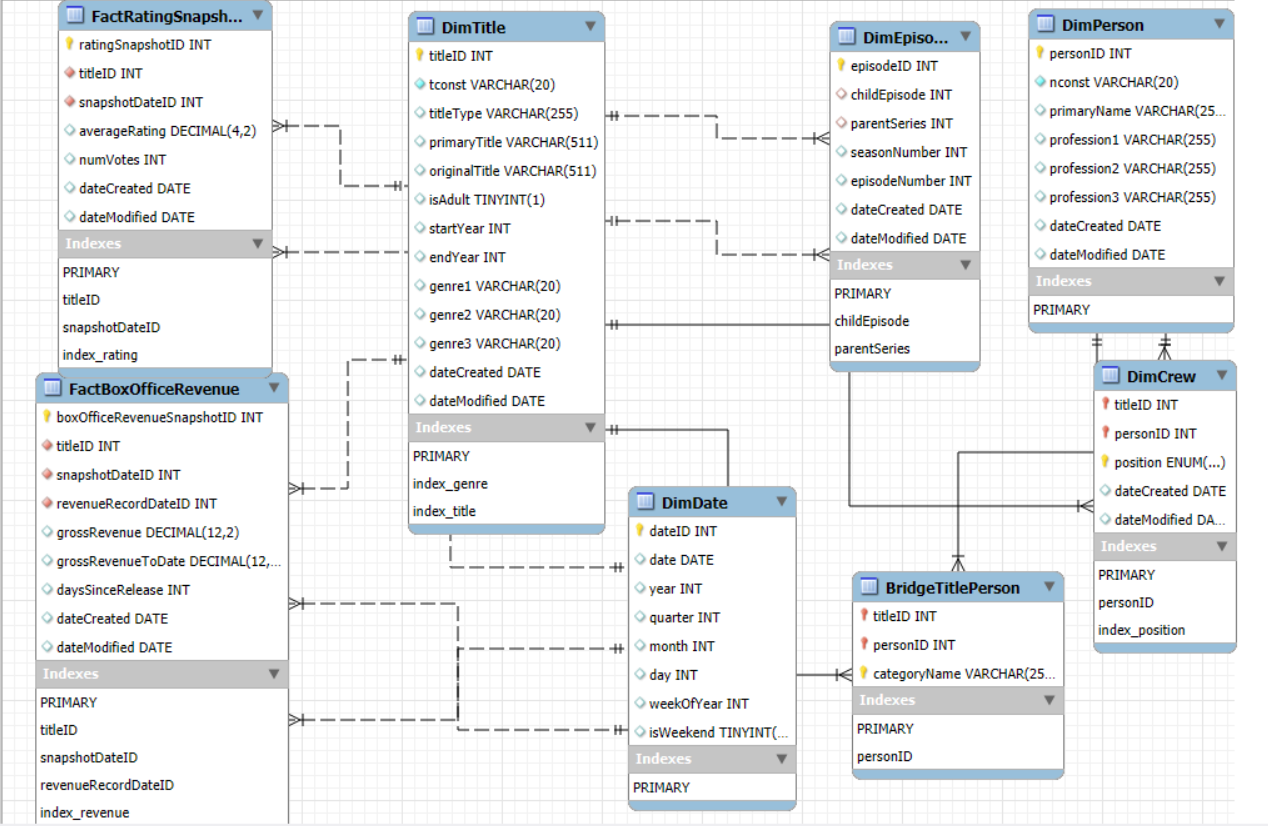
\includegraphics[width=0.8\linewidth]{images/schema.png}
    \caption{Schema for the OLAP Application}
    \label{fig:your_label}
\end{figure}

\subsubsection{Indexes}

Indexes are used in order to query results efficiently and is an essential tool in improving query performance. In the purposes of our OLAP application that analyzes rating, revenue, and genres, it was imperative that we create secondary indexes on these columns to decrease the runtime significantly. 

\begin{lstlisting}
CREATE INDEX index_position
ON DimCrew (position)

CREATE INDEX index_genre
ON DimTitle (genre1, genre2, genre3)

CREATE INDEX index_title
ON DimTitle (titleType)

CREATE INDEX index_rating
ON FactRatingSnapshot (averageRating)

CREATE INDEX index_revenue
ON FactBoxOfficeRevenue (grossRevenueToDate)
\end{lstlisting}

\subsubsection{Query Restructuring}

The queries we had used in our application had numerous optimizations, restructuring, and formatting for readability. CTEs were used throughout majority of the queries for formatting alongside the inner queries being the most selective to return the least amount of rows as possible. Doing this decreases the query runtime and allows us to retrieve thousands to tens of thousands in a sea of tens of millions of rows in mere seconds. Additionally, operations such as only selecting required columns, aggregates and early filtering proved to be effective in further decreasing the runtime to strive for the most optimized query runtime as possible.

\begin{lstlisting}
WITH Movies(titleID) AS ( 
        SELECT dt.titleID
        FROM DimTitle dt
        WHERE dt.titleType = 'movie'
    )
SELECT 
    SUM(fbor.grossRevenue) / 1000000 
        AS totalRevenueThatDayInMillions, 
    dd.year, 
    dd.month, 
    dd.day
FROM Movies m
JOIN FactBoxOfficeRevenue fbor 
ON fbor.titleID = m.titleID
JOIN DimDate dd 
ON dd.dateID = fbor.revenueRecordDateID
WHERE dd.year = "2024"
GROUP BY dd.year, dd.month, dd.day
ORDER BY dd.year, dd.month, dd.day;
\end{lstlisting}

Such example shows that the table for Movies is much more readable since it is contained in the CTE rather than being  stored in a subquery.

\subsubsection{Optimization at Hardware Level}

Alongside database design, indexes, and query restructuring, providing an appropriate amount of hardware resources is another important point of focus as the CPU, RAM, and storage are important aspects of querying operations. The database server contains 4 cores, 12GB of RAM, and 64GB of disk storage to store the entire IMDB dataset.

    \section{Results and Analysis}

    \section{Conclusion}

In this project, we have created an OLAP application using database warehouse techniques such as ETL, indexing, query optimization and presented data in a manner that is easily
appealable to clients or users that want to gain a deeper understanding as to how to a movie's rating or revenues tie in to several different factors such as release dates, directors, 
and genres. \\

The importance of building a database warehouse is to make data-driven decisions through thorough analysis. Additionally, it is also used to store and keep historical data such as the
\texttt{FactRatingSnapshot} table which contains historical ratings of each and every movie and TV show within IMDB. Using this data warehouse, we are able to preserve history and
the moments that get snapshotted between the data. A data warehouse is not just a database for pure analysis, it's also important to remember that it contains history as we know it. \\

Preparing the data warehouse would not have been possible without our ETL script. The ETL script first extracts data from its sources periodically to update new information into the data
warehouse. Following the first step, the script then transforms the data to data that conforms to the schema and purpose of the OLAP application. Doing this enables us to keep our
analytical queries functioning to allow us to continuously update the data we retrieve to make sure our analysis is always up to date and that we are able to store the data properly.
Lastly, the last step involves the loading of the data into the warehouse itself in order to preserve the data to be stored and used in the application itself. \\

The purpose of an OLAP is to be able to store and analyze data. An OLTP is a venue of retrieving, updating, and displaying data that should be quick and efficient. On the other hand, the
OLAP extracts and uses the data from an OLTP to make data-driven decisions. These data-driven decisions are used to help companies and large corporations make smart and informed decisions
that allows their companies to perform large-scale operations and develop important business strategies. \\

Additionally, these decisions need to be made quickly as time is money for these large companies. This brings us to the important of query optimization as being able to analyze data
efficiently and effectively will put a corporation's business far ahead of its competitors. Therefore, query optimizations such as database design, indexes, query restructuring, and
even optimizations at the hardware level are all optimization strategies that these companies use to analyze their data as quickly as possible. \\

However, not all these optimization strategies can be used without thought. For example, indexes should be used if the column is used throughout multiple queries and is used as a basis
for rows in GROUP BY, ORDER BY, JOIN, and WHERE operations. Using indexes carelessly may cause for concern as retrieving new data will cause the data warehouse to consistently update
its index and would even detriment the storage space of the data warehouse. \\

While doing this project, our group had learnt and experienced multiple different aspects of database warehouse concepts and the deeper theory behind it. These include preparing an ETL
script, migrating millions of rows on data, making database design decisions based on data profiling and domain knowledge, understanding how CPU cores work during reading and writing data,
making readable and highly optimized queries, and so much more. Due to the develop of our application, we can now provide our users valuable insights and information as to what defines a
movies rating and revenue whether it be the release date, genre, or director associated with the film. To other database developers, we set an example as to that even students are able to
transform a large scale database like IMDB's into our own OLAP application that we can gain valuable insights out of. 
    
    \section{References}

    \section{Declarations}

\subsection{Declaration of Generative AI in Scientific Writing}

During the preparation of this work, the authors used GitHub Copilot and Claude AI to assist with the following tasks: code completion and syntax suggestions during SQL script development, debugging MySQL configuration issues, generating boilerplate code for the Next.js OLAP application, and structuring sections of the technical report. After using these tools, the authors reviewed and edited the content as needed and take full responsibility for the content of this publication.

\subsection{Record of Contribution}

\textbf{Clarence Ivan Ang}.  Developed the OLAP application frontend using Next.js and React, contributed with Malks Mogen David with designing the analytical modules for the OLAP application, and wrote the Introduction, OLAP Application, and Query Processing sections of the technical report.

\textbf{Clive Jarel Ang}.  Designed the staging area and data warehouse, implemented the dimensional model structure including fact and dimension tables, developed the ETL transformation logic for IMDb datasets, optimized MySQL configuration for large-scale data loading, and wrote the Introduction, Data Warehouse, and ETL Script sections of the technical report.

\textbf{Malks Mogen David}.  Developed the OLAP application backend using Next.js and React, contributed with Clarence Ivan Ang with designing the analytical modules for the OLAP application, and wrote the OLAP Application and Query Processing sections of the technical report.

\textbf{Rinaldo Adelrico Lee}.  Contributed to the overall system architecture design, implemented the data validation and quality checks, conducted performance testing and optimization of ETL processes, and wrote the Results and Analysis, and Conclusion sections of the technical report.

\bibliographystyle{ACM-Reference-Format}
\bibliography{sources}

\appendix

    \section{Appendices}

\end{document}